\chapter{A finite volumes code}
\label{section:python-api-examples:finite-volumes}

We create a simple Finite Volumes solver here.
The examples starts with a simple regular grid, parallelises this grid, and
finally adds adaptive mesh refinment (AMR).
It employs a block-structured formalism and relies heavily on premanufactured
actions and solver ingredients from the ExaHyPE2/ExaClaw project.


\section{Setting up the data structures}

We model our grid as an AMR grid consisting of $N \times N$ blocks.
We call these blocks \emph{patches}.
In the example below, we have chosen $N=7$.
In general, odd choices of $N$ are advantageous once you enable AMR as we will
discuss later.

\begin{center}
  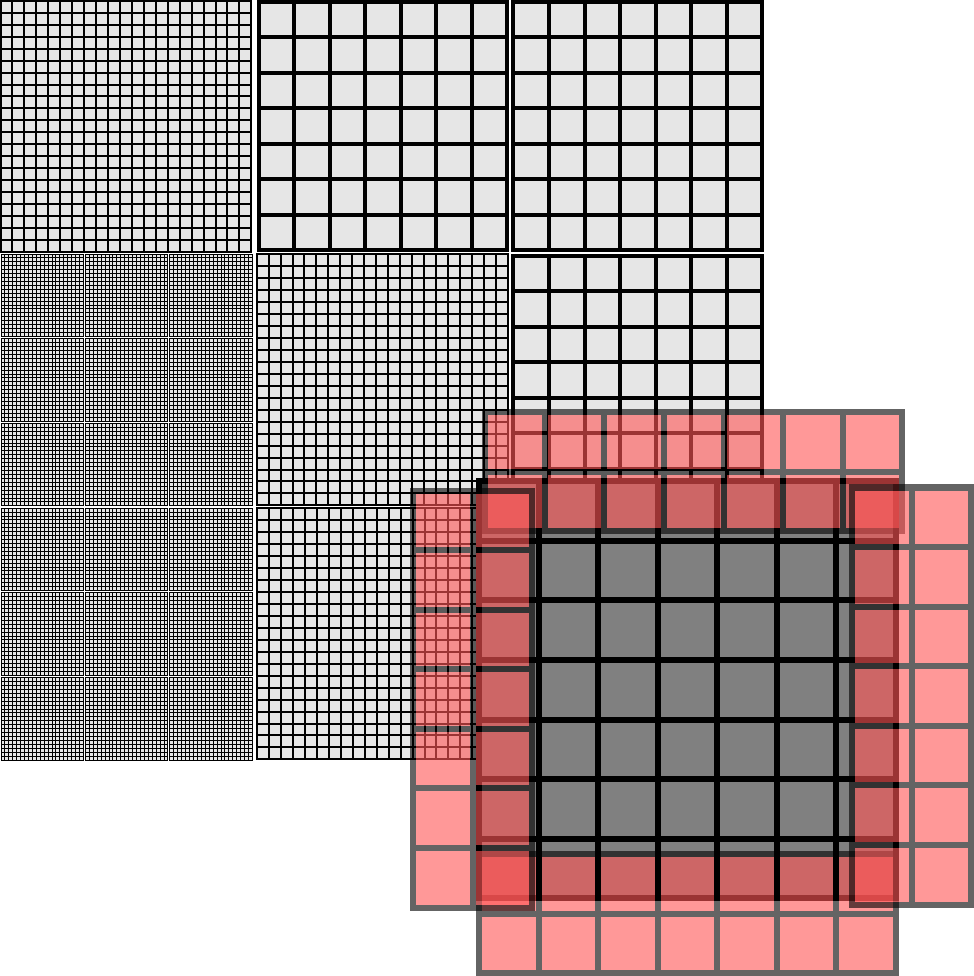
\includegraphics[width=0.6\textwidth]{42_finite-volumes/block-structured.pdf}
\end{center}

\begin{code}
project = peano4.Project( ["examples", "finitevolumes"], "." )
patch_size = 7
unknowns   = 5
patch = peano4.datamodel.Patch( (patch_size,patch_size,patch_size), unknowns, "Q" )
project.datamodel.add_cell(patch)
\end{code}

\noindent
In the above example, every voxel within the $N \times N$ patches holds five
unknowns.
In general, I prefer the term voxel here, as cell again is ambigous given that
we construct the Peano4 host mesh from cells.


With one patch per cell, we could traverse the mesh and do something per cell.
This however is of limited value.
We have to couple the phenomena what is going on in neighbouring cells.
Peano realises a strict element-wise traversal, i.e.~there's no way to access
the neighbour cell of a cell directly.
However, we can hijack the faces.


The idea here is that we embed a $2 \times N$ ($d=2$) or $2 \times N \times N$
($d=3$), respectively, patch into each face. 
Let this auxiliary patch overlap the adjacent cells.
Then, we effectively have a halo of one cell available within each cell:
We know the cell data. 
We also have access to the $2d$ faces where each hosts a degenerated patch.
One later of this patch is a copy of our own data, i.e.~does not give us
additional information.
The other layer of the auxiliary patch however holds data from the neighbour.
It gives us information from the neighbour patch.


In theory, we could only replicate those quantities that we really need. 
But it makes our live easier to just hold all five quantities in the auxiliary
face data structures, too:

\begin{code}
patch_overlap = peano4.datamodel.Patch( (2,patch_size,patch_size), unknowns, "Q" )
project.datamodel.add_face(patch_overlap)
\end{code}


Before we generate the code, we export some of the Python constants that we use
into C/C++, so we have it available there, too:

\begin{code}
project.constants.export( "PatchSize", patch_size )
project.constants.export( "NumberOfUnknownsPerCell", unknowns )
\end{code}


All the stuff we use, we use the toolbox and some vis

% 
% import peano4.visualisation
% import peano4.toolbox
